\documentclass{article}
\usepackage{xcolor}
\usepackage{graphicx,amsmath,amssymb}
\newcommand{\myname}{Mark Taylor}

%---------------------- My article content----------------------
\linespread{1.5}
\begin{document}

\pagecolor{pink}
\begin{center}
{\Huge \textcolor[rgb]{0.1,0.3,1}{\textit{Splinetool usage summary } }}\\[5mm]
10170437 \myname\\
Oct. 6, 2019\\[20pt]
\end{center}

Well, there are quite a few options about splinetool $\texttt{\emph{MATLAB}}^\circledR$ program when we first enter
the graphical user interface (GUI)  manu,  including the option of importing some data from your workspace, which is
real very convenient \&  impressive.\quad Here I am mainly talk some some about \textbf{Import your own data} option.
The rest parts , for example Titanium heat data, Census data, Richard Tapia's drag race data, are some distinct aspects in
which the spline fitting applies.\par

OK, first, let's see the home window (see \texttt{figure 1})  if you use those default data input options.
We can do many a  manipulation on the fitting curves, well, in the \texttt{View} bar we can
choose  \texttt{Show 1st Derivative, Show 1st Derivative, Show Error}  modes, in which cases the
shape of the lower curve may alter when we attempt to modify (add or delete point) the data
through \texttt{Edit} bar on the top. You can also turn grid on in the \texttt{Tool} bar if you like .\par

Then, let's proceed to the interesting parts. On the top we can see the \texttt{List of approximation} box,
we first replicate a spline curve, you know, just do a copy, for the sake of comparison.  After that,
let's focus on the middle box \texttt{Approximation method} where we get lots of options to manipulate
the curves. We have following 4 kinds of method provided by this program: \texttt{Cubic Spline
Interpolation}, \texttt{smoothing Spline}, \texttt{Least-Square Approximation}, and \texttt{Spline Interpolation}.
When we select the \texttt{Cubic Spline Interpolation} method, bellowing we get corresponding \texttt{End condition}
which includes options: \texttt{not-a-knot, clamped, complete, second, periodic, variational,
natural, Lagrange, Custom}. In our text, we have learned boundary  conditions
like clamped boundary (s'(a)=s'(b)), natural boundary (s''(a)=s''(b)=0),
periodic boundary (s''(a)=s''(b)).  The other 3 methods correspond with \texttt{Order} options below
methods options. Take Last-Square Approximation for example, as the order increases,
the spline becomes more smooth and error is decreasing exponentially! (see \texttt{figure 2}
and \texttt{figure 3}). Last, in the bottom box you slowly increase (decrease)  weights to
see error varies graphically. You can also turn on \texttt{Breaks} which enable you see many vertical
lines that intersect the spline at those data points (see \texttt{figure 4}). At the very bottom of this program
box, you can see the \texttt{Bottomline}  which tells you that the toolbox function csape was used to create the spline.


%---------------pictures-------------------
% fig1
\begin{figure}
\centering
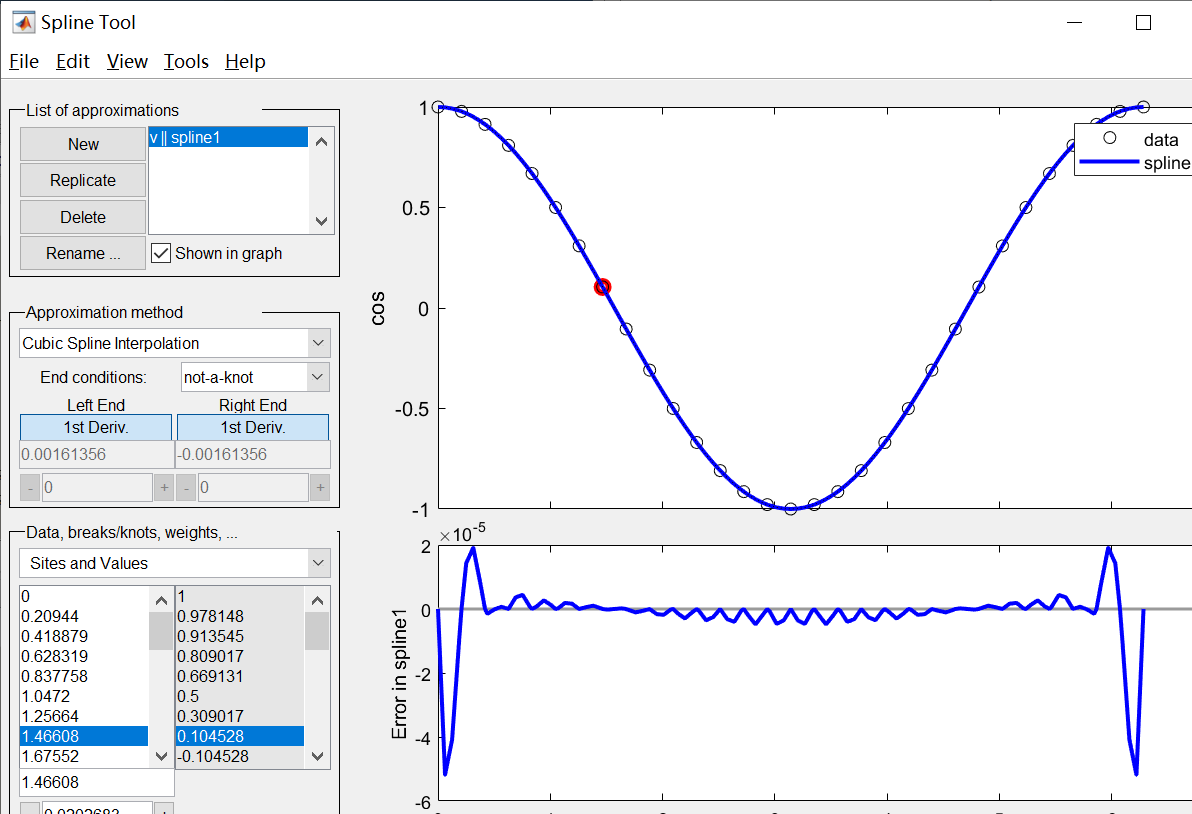
\includegraphics[width=10cm]{img/default_home_window.png}
\caption{Default initial window}
\end{figure}

% fig2
\begin{figure}
\centering
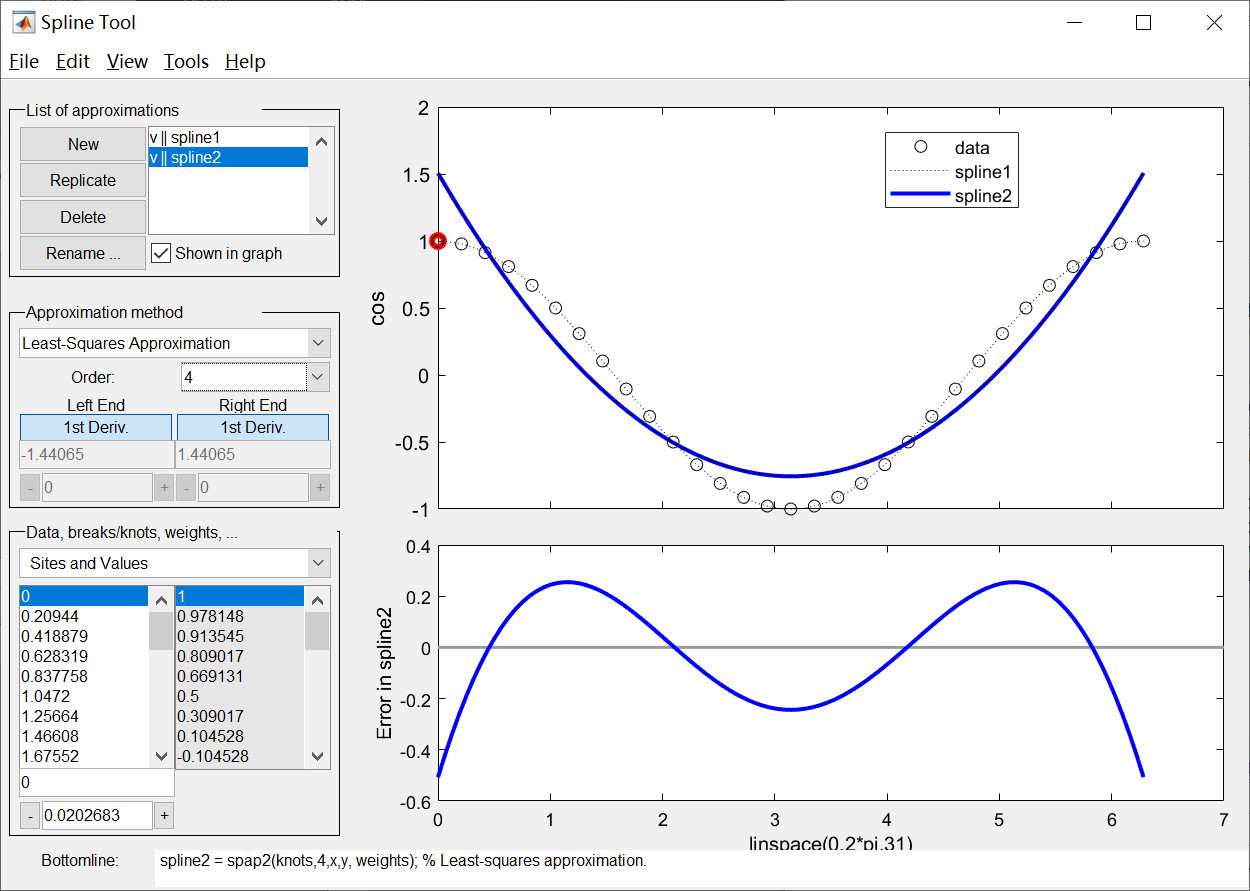
\includegraphics[width=10cm]{img/Last-Square_Appr4.jpg}
\caption{Last-Square Appr order 4}
\end{figure}

% fig3
\begin{figure}
\centering
\includegraphics[width=10cm]{img/Last-Square_Appr9.jpg}
\caption{Last-Square Appr order 9}
\end{figure}

% fig4
\begin{figure}
\centering
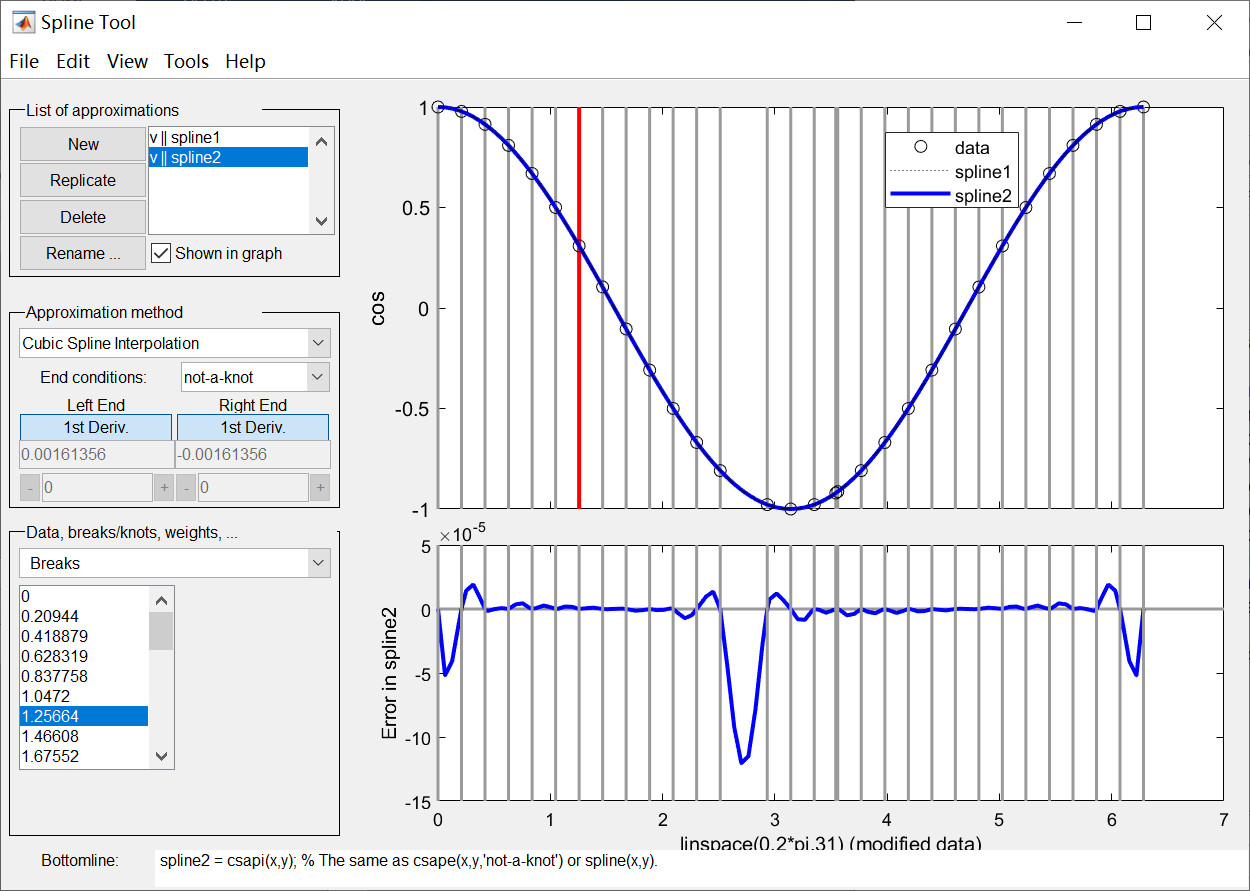
\includegraphics[width=10cm]{img/breaks_mode.jpg}
\caption{Breaks mode}
\end{figure}

OK, now, it's our shot. Well, we first create a \texttt{Splinetool} test function, say $\frac{sin(x)}{x}$ (see \texttt{figure 5}),
create one whichever you like. Oh, there is a break point x=0, and the program gives us a warning, click OK to ignore it,
and here comes our home window (see \texttt{figure 6}).Then we can play around with those buttons.
For instance, we replicate one and then select the \texttt{Least-Square Approximation} method, you'll get a terrible match,
and when you ascend the order, it becomes better(see \texttt{figure 7} and \texttt{figure 8}).
The other 3 spline methods have almost identical effect in drawing the fitting curves.

% fig5
\begin{figure}
\centering
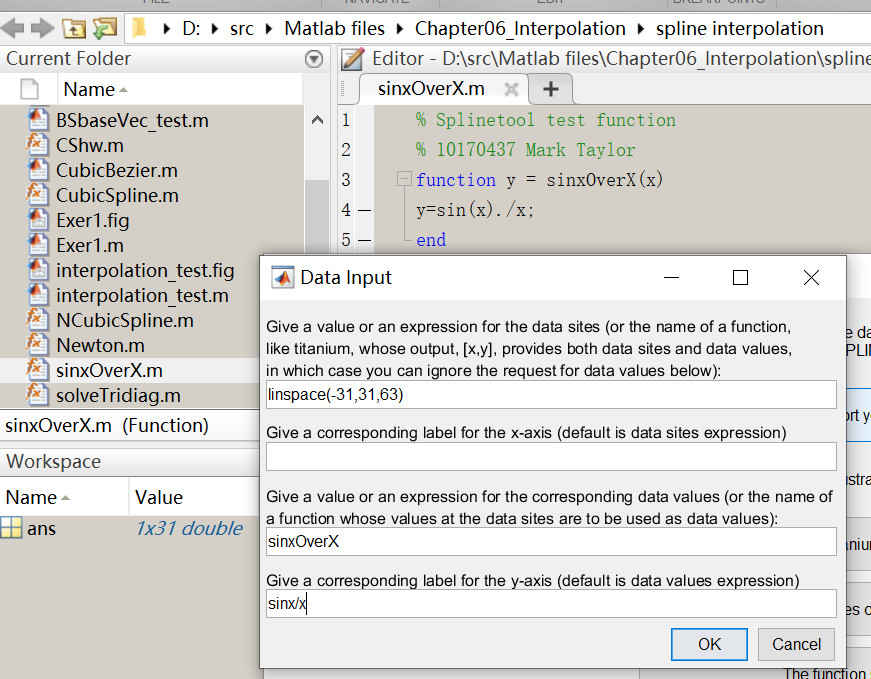
\includegraphics[width=10cm]{img/my_shot_input.jpg}
\caption{My data input}
\end{figure}

% fig6
\begin{figure}
\centering
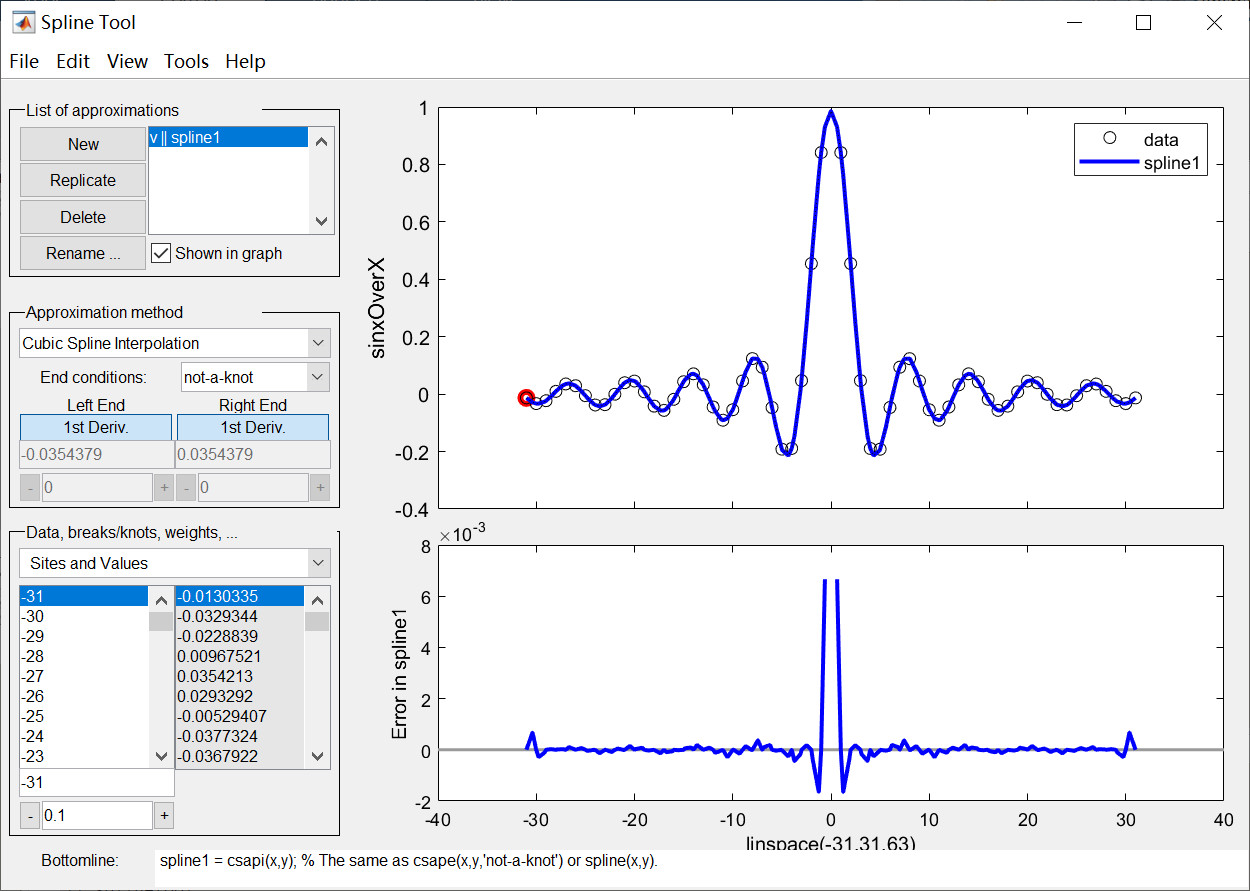
\includegraphics[width=10cm]{img/My_shot_window.jpg}
\caption{sinx/x  initial window}
\end{figure}

% fig7
\begin{figure}
\centering
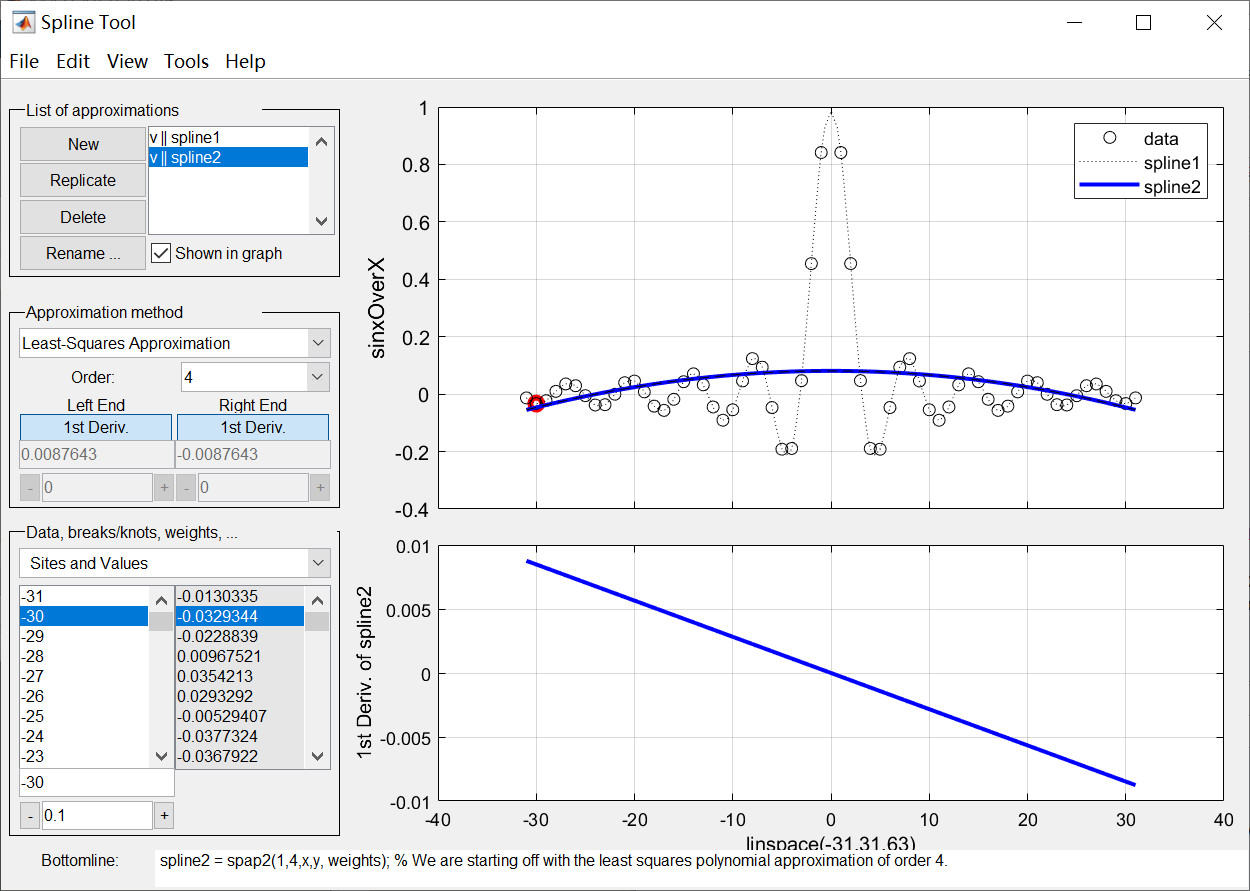
\includegraphics[width=10cm]{img/bad.jpg}
\caption{Last-Square Appr, bad }
\end{figure}

% fig8
\begin{figure}
\centering
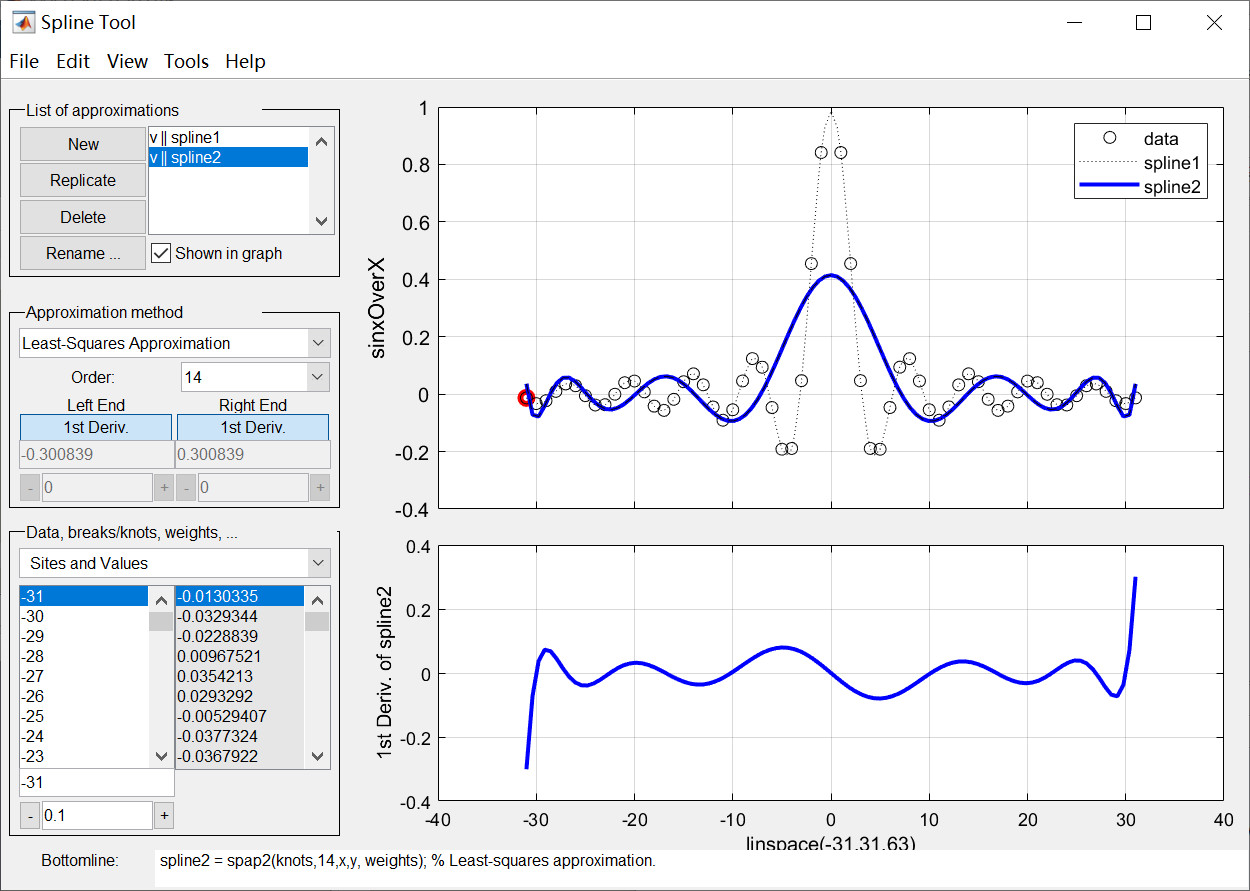
\includegraphics[width=10cm]{img/better.jpg}
\caption{Last-Square Appr, better}
\end{figure}

\end{document}
